\chapter{ATLAS トリガーシステム}\label{chapter3}
ATLAS実験では陽子陽子衝突が$\SI{40}{MHz}$で起こるので、すべての事象に対して処理を行い、記録することは不可能である。
そのため、膨大な数のデータの中から興味のある事象のみを選別して保存している。このシステムは「トリガーシステム」と呼ばれる。

以下でATLAS実験におけるトリガーシステムの概略とミューオントリガーシステムについて詳しく述べる。

\section{ATLASトリガーシステムの概要}\label{chapter3-1}
トリガーシステムは測定したい物理に対してミューオン、電子、光子、タウ、ジェットなどの種類が用意されている。
事象の選別では、横運動量やエネルギーに対して閾値を設けて、単位時間当たりに処理するイベントの数~(トリガーレート)が処理能力、記憶装置などの計算資源を超えないようにしている。

ATLAS実験ではこのトリガーシステムは2段階で構成されている。
ハードウェアを用いて高速演算を行う初段トリガー~(Level-1~trigger,~L1)とソフトウェアを用いて精密処理を行う後段トリガー~(High~Level~trigger,~HLT)である。
L1では一部のトリガー用検出器の情報を用いて高速に処理を行い、粒子のエネルギーや運動量、位置を素早く大まかに算出することで膨大なレートを削減している。
次の段階であるHLTでは、L1の情報をもとに精密用検出器の情報を用いてより精密な飛跡再構成とトリガー判定を行う。
これによって、トリガーレートはL1で約$\SI{100}{\kHz}$まで、HLTで約$\SI{1}{\kHz}$程度まで削減され、大容量記憶装置に記録される。

図~\ref{fig:3-1}にトリガーシステムの概要を示す。

\begin{figure}[H]
  \centering
  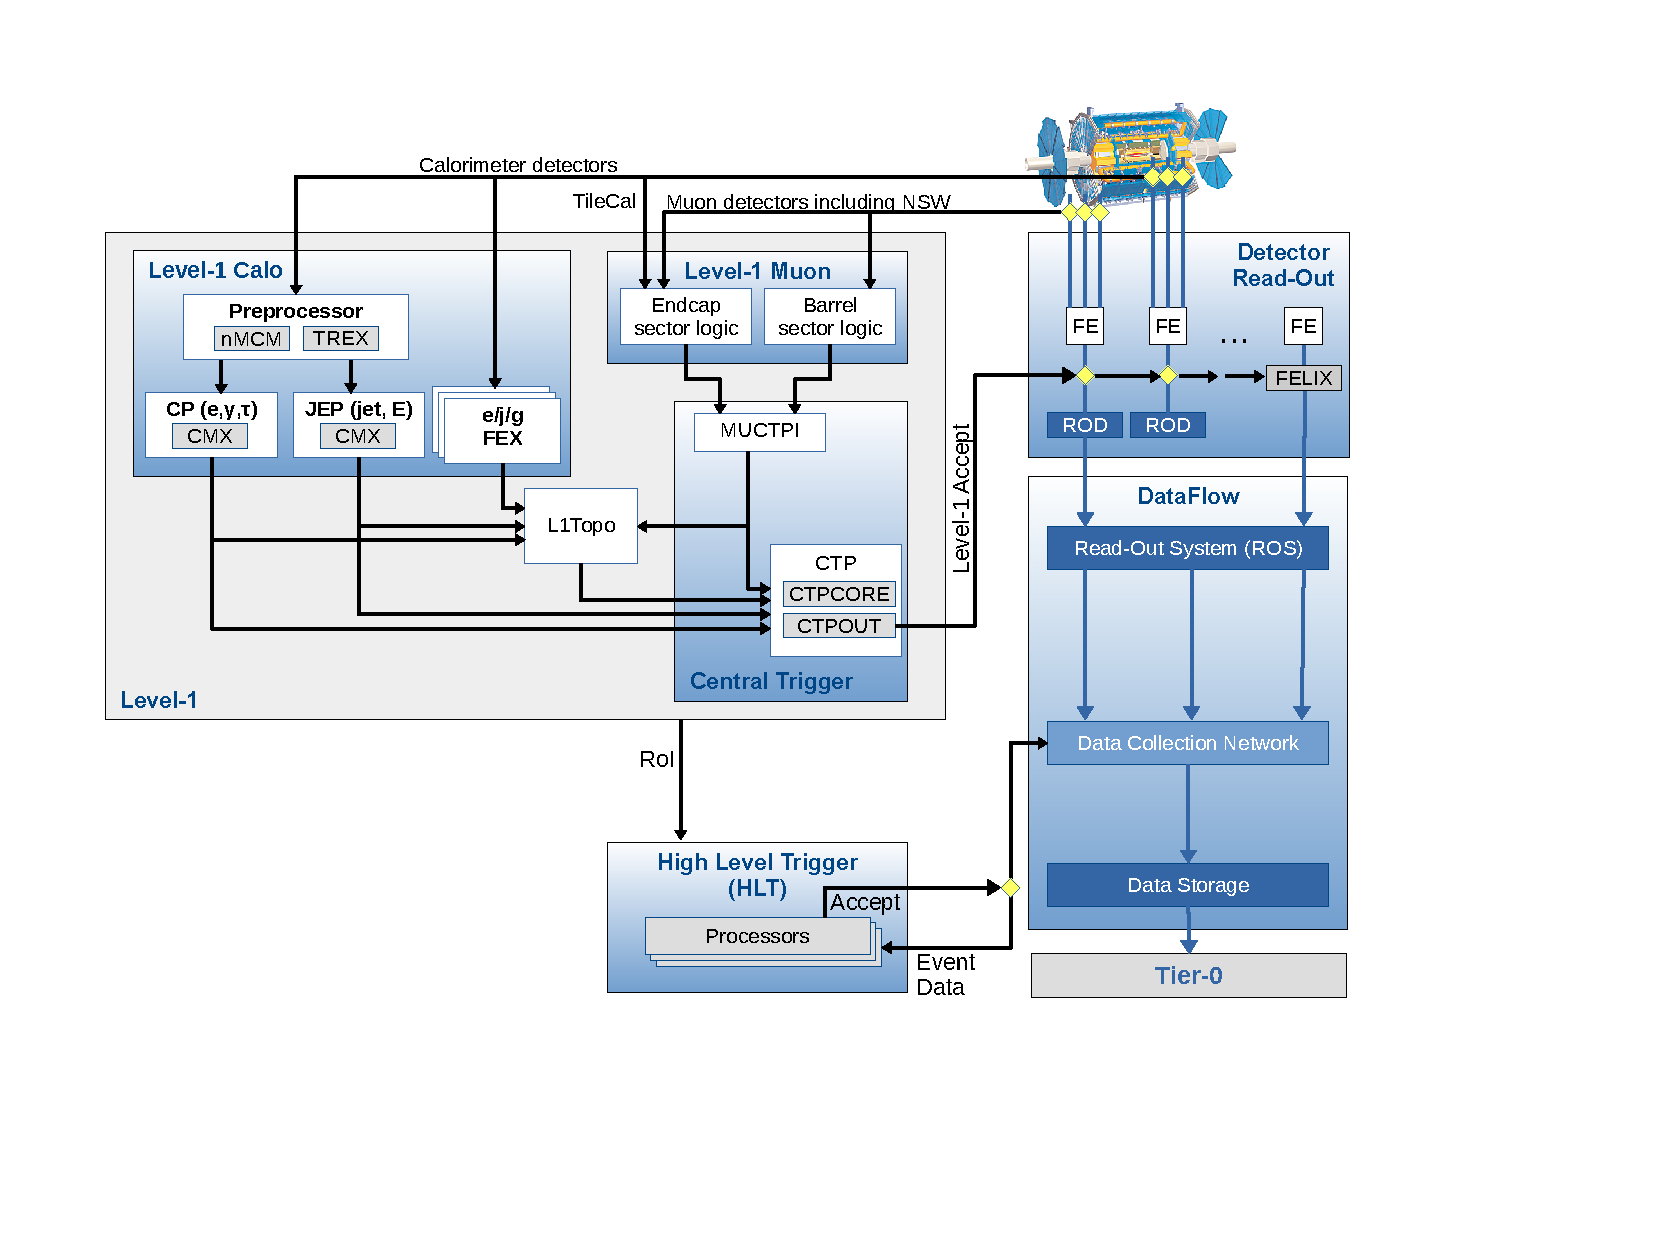
\includegraphics[clip, width=14cm]{fig/3/tdaq-run3-schematic.pdf}
  \caption{ATLASトリガーシステム全体のデータフロー\cite{article:approvedPlotsDAQ}。}
  \label{fig:3-1}
\end{figure}

本論文では、トリガーとしてミューオンを用いるミューオントリガーを扱う。
ミューオントリガーでは、事象中に存在するミューオンの個数と、それぞれのミューオンの$\pt$の値に対して閾値が定められており、それぞれ一定値以上である場合にトリガーが発行される。


\section{ミューオントリガーシステム}\label{chapter3-2}
図~\ref{fig:muonTrigger}にミューオントリガー全体のデータの流れを示す。

\begin{figure}[H]
  \centering
  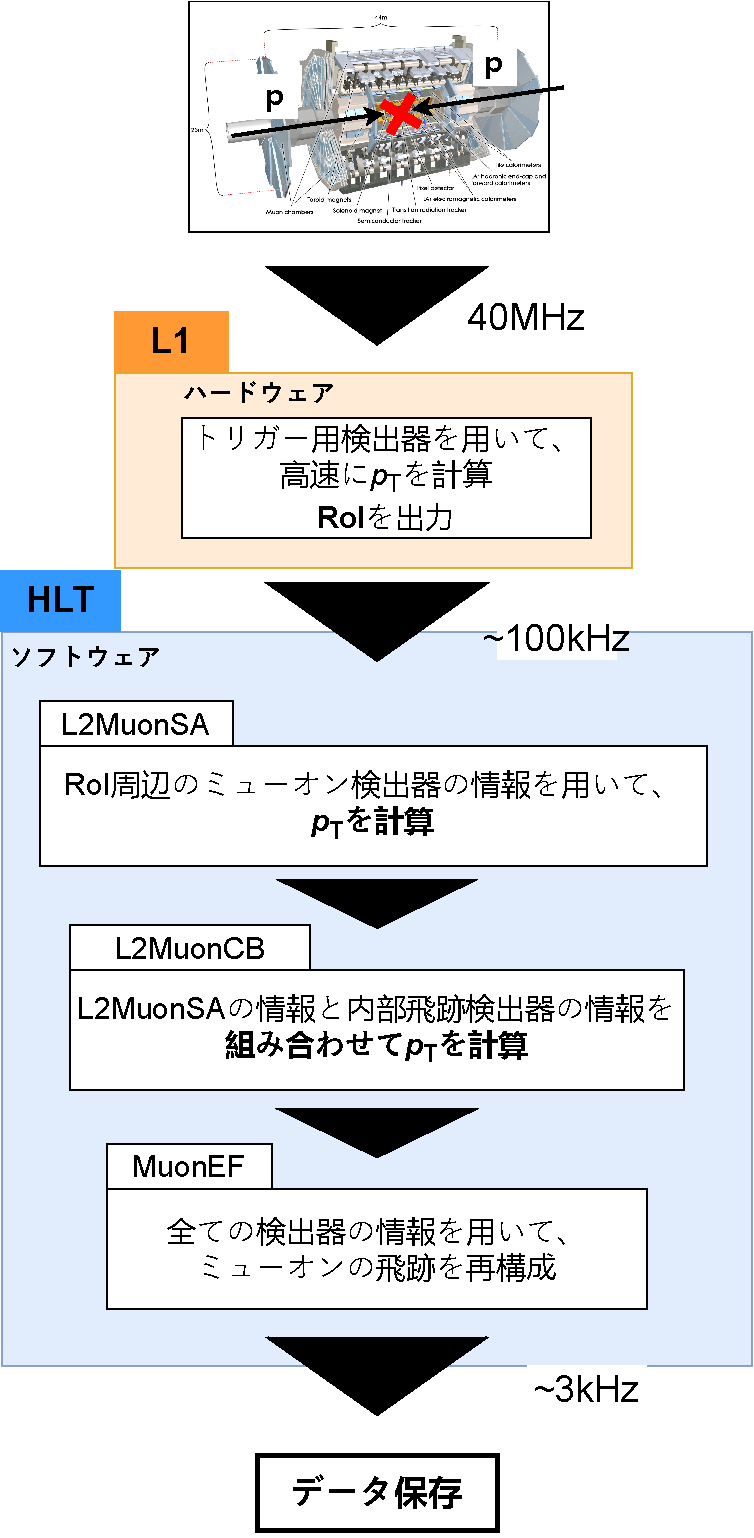
\includegraphics[clip, width=8cm]{fig/3/muonTrigger.pdf}
  \caption{ミューオントリガーのデータフロー。}
  \label{fig:muonTrigger}
\end{figure}

L1ではトリガー判定を行い判定をクリアしたミューオンに対して、大まかなミューオンの通過位置を示す~Region~of~Interest~(RoI)を発行する。
HLTではL1から送られてきた~RoIが持つ$\eta$、$\phi$の情報をもとに、RoI周辺の検出器の情報を用いて部分飛跡の再構成を行い、飛跡から求めた$\pt$に対して閾値を設けることでトリガー判定を行う。

HLTでは複数の段階で飛跡から運動量を再構成している。
まず~RoI周辺のミューオン検出器の情報のみを用いてミューオンの部分飛跡を求め、その組み合わせで運動量を再構成する~Level-2~StandAlone~muon~trigger~(L2MuonSA)、次にL2MuonSAの情報と内部飛跡検出器の情報を組み合わせることによってより正確な飛跡の再構成と$\pt$の計算を行う~Level-2~Combined~muon~trigger~(L2MuonCB)、最後にここまでで選別されてきた事象に対して全検出器の情報を用い、オフライン再構成と同等のアルゴリズムを用いることで正確に$\pt$を計算し、トリガー判定を行う~Event~Filter~(MuonEF)の3段階である。
以下でそれぞれのアルゴリズムの詳細について述べる。

\subsection{初段トリガーシステム~(Level-1 Trigger)}\label{chapter3-2-1}
ここでは、L1トリガーについて、バレル領域とエンドキャップ領域それぞれについて説明する。
図~\ref{fig:3-2}にバレル領域、エンドキャップ領域それぞれでの~L1ミューオントリガーアルゴリズムの概念図を示す。

\begin{figure}[h]
  \centering
  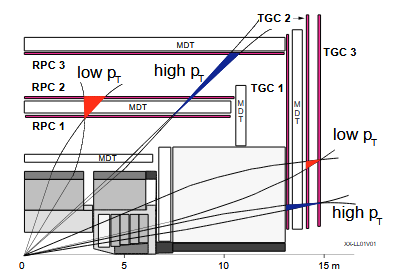
\includegraphics[clip, width=13cm]{fig/3/muon_trigger_overview.png}
  \caption{L1ミューオントリガーの概念図\cite{article:barrelSystem}。}
  \label{fig:3-2}
\end{figure}

\subsubsection{バレル領域}
バレル領域では~RPCのヒット情報を用いてミューオンの再構成を行う。2章で述べたように~RPCはミドルステーションに~RPC1と~RPC2の2層、アウターステーションに~RPC3の1層の合計3層が配置されている。RPCのそれぞれの層は、$\eta$、$\phi$方向の測定を行うために$\eta$--stripと$\phi$--stripを重ねたダブレット構造のストリップ層が2層で構成されている。
トリガーアルゴリズムは、以下の通りである。
まず~RPC2にヒットがあることを要求し、このヒットの点と衝突点を結ぶ直線を探索領域~(ロード)の中心として定義し、ロード内にある~RPC1のヒットを探索する。探索領域の幅は要求する$\pt$閾値によって決まる。$\pt$しきい値が高いときのみ~RPC3のヒットも用いる。
これはミューオンはトロイド磁石によって$\eta$方向に曲げられ、高い$\pt$を持つミューオンほど磁場で曲げられず衝突点から真っ直ぐ飛び~RPC3を通過しやすくなるからである。
低い$\pt$を持つミューオンのトリガー判定はRPC1とRPC2で行い、高い$\pt$を持つミューオンのトリガー判定は~RPC1と~RPC2、RPC3で行う。

この領域におけるL1トリガーは、$\eta$、$\phi$方向にそれぞれ32分割された合計64分割のそれぞれ独立なトリガーセクターごとに判定が行われる。図~\ref{fig:3-3}にその概略を示す。
さらに各セクターはその内部がおおよそ$\Delta\eta\times\Delta\phi=0.2\times0.1$、$\Delta\eta\times\Delta\phi=0.1\times0.2$の大きさ~Coincidence~matrix($\eta$-CM、$\phi$-CM)に区分され、このCM単位で~RPC1と~RPC2または~RPC2と~PRC3のコインシデンスを取り、$\pt$の閾値の判定を行う。
隣接する2つずつの$\eta$-CM、$\phi$-CMはまとめて~Padと呼ばれる。このPadは$\eta\times\phi=0.2\times0.2$の大きさで、ミューオンの通過領域を表す~RoIが4つで構成される。RoIは$\eta$--CM、$\phi$--CMが重なる$\eta\times\phi=0.1\times0.1$の大きさの領域であり、ハードウェアの制限により~Pad1つに付き最大1つしか定義できない。L1で定義した~RoIの情報は後段ミューオントリガーに送られる。

\begin{figure}[h]
  \centering
  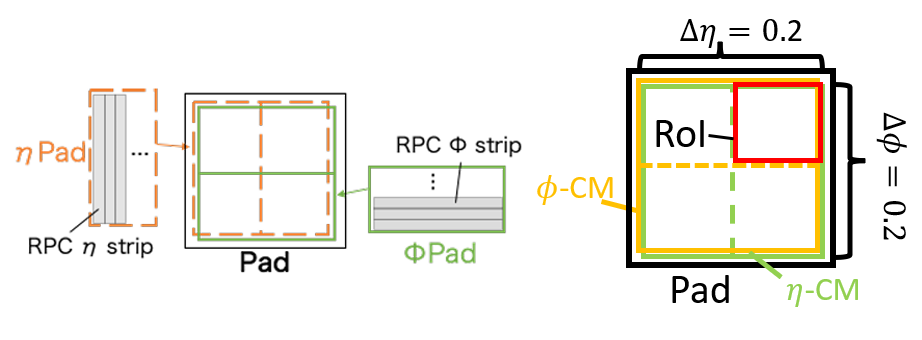
\includegraphics[clip, width=13cm]{fig/3/L1_RoI_CM.png}
  \caption{バレル領域における~Padと~RoI、Coincidence~matrix~(CM)の概念図。}
  \label{fig:3-3}
\end{figure}

\subsubsection{エンドキャップ領域}
エンドキャップ領域では2章で示したTGCのヒット情報を用いてミューオンの再構成を行う。
TGCはインナーステーションに1枚~(I)、ミドルステーションに3枚~(M1、M2、M3)配置されている。
トリガーアルゴリズムは以下の通りである。
まずM3にヒットがあることを要求し、M3のヒットと衝突点を結ぶ直線のロードの中心として定義する。ミューオンは検出器より内側のトロイド磁場によって曲げられてTGCに入射するので、図~\ref{fig:3-4}のようにM1において実際のヒット点と直線は~dR、d$\phi$だけずれる。
あらかじめ作成されている~dR、d$\phi$と$\pt$の対応関係を示した~Coincidence~Window~(CW)図~\ref{fig:3-5}を用いて、~dR、d$\phi$から$\pt$を計算することで短時間での$\pt$判定を行っている。

\begin{figure}[h]
  \centering
  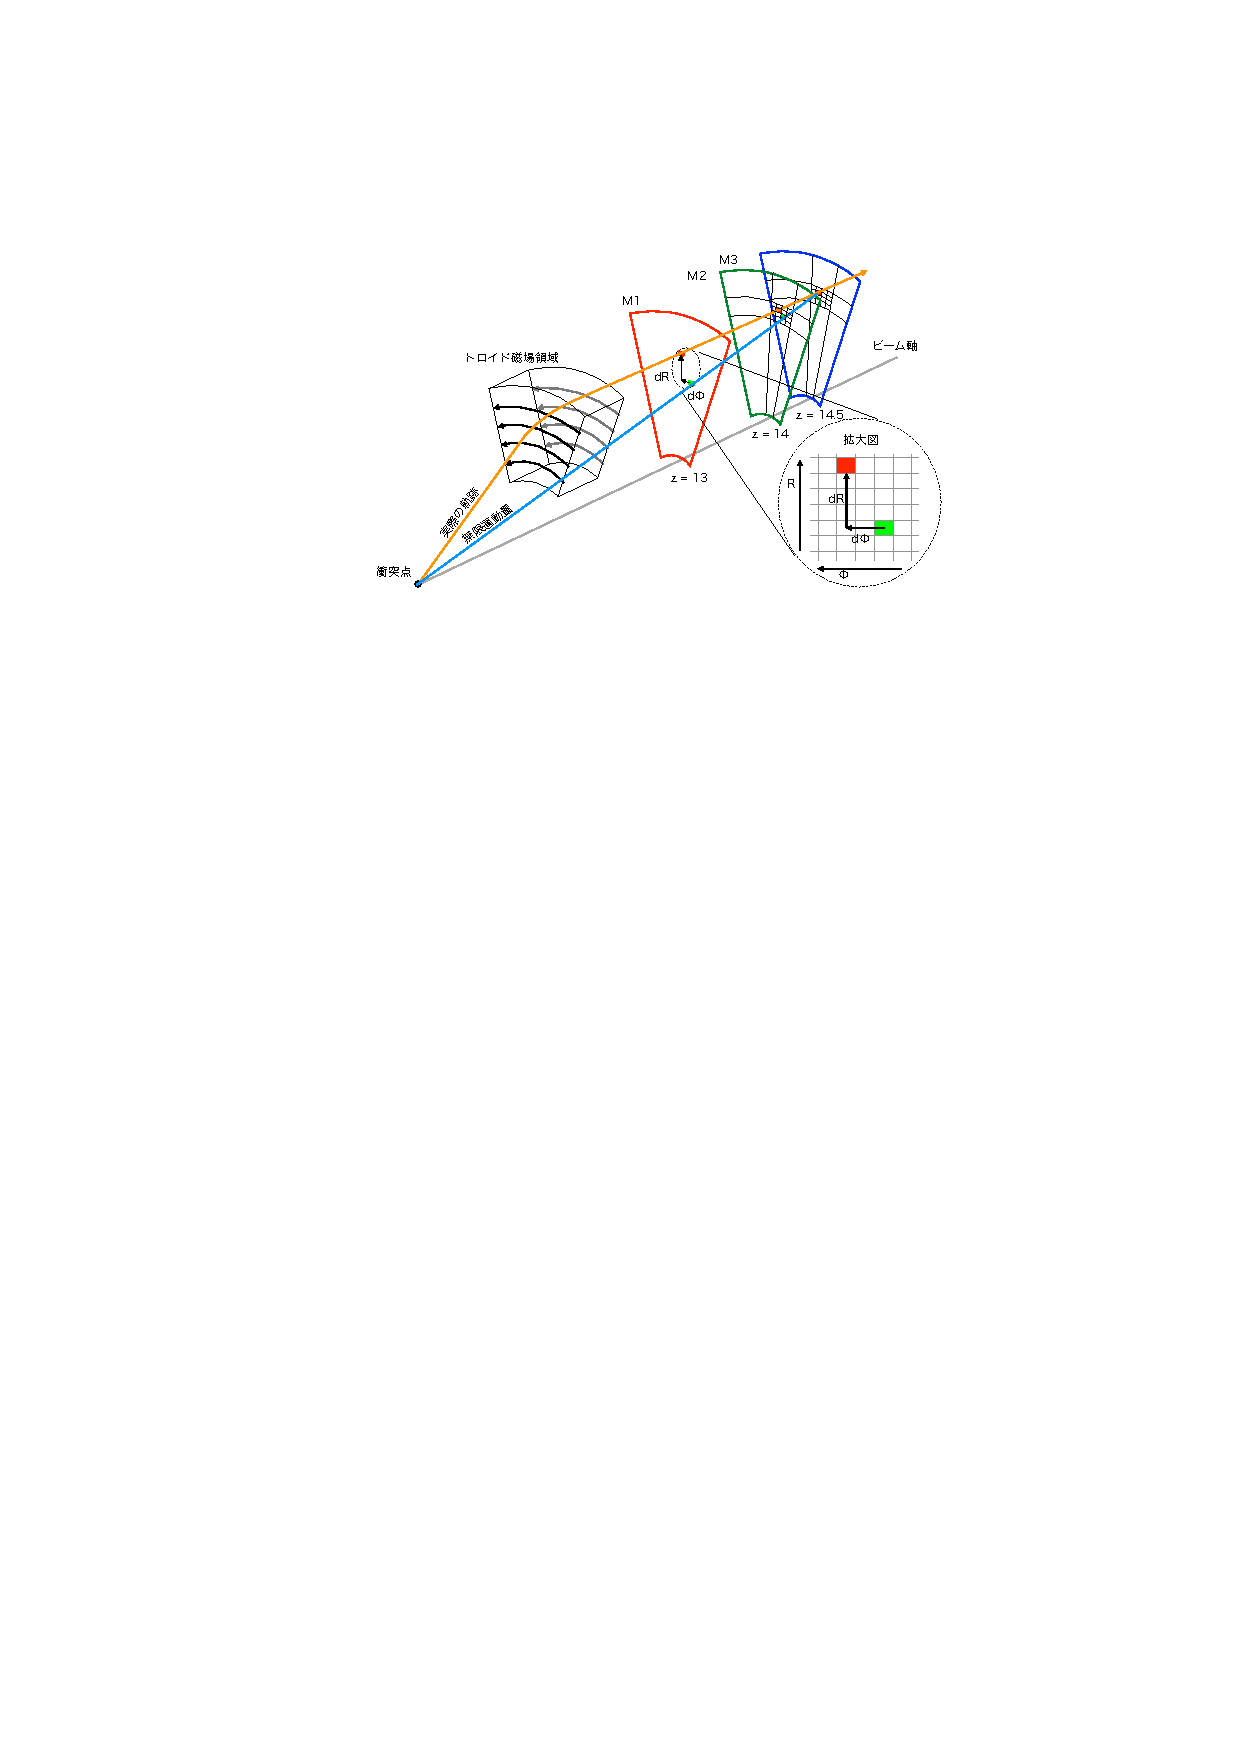
\includegraphics[clip, width=12cm]{fig/3/akatsuka_mt_trigger_scheme.pdf}
  \caption{M3TGCと衝突点を結ぶ直線と実際の飛跡の~M1TGCでのずれとdR、d$\phi$の概念図\cite{article:akatsuka}。}
  \label{fig:3-4}
\end{figure}

\begin{figure}[h]
  \centering
  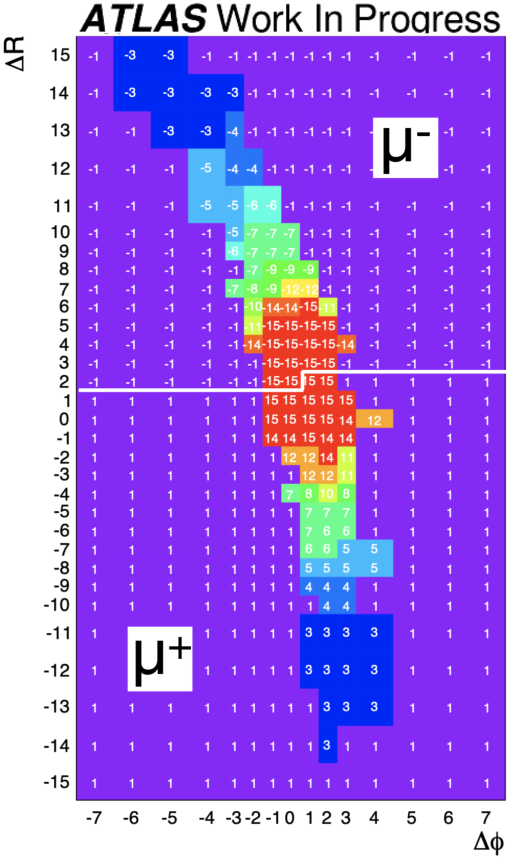
\includegraphics[clip, width=8cm]{fig/3/Run3CW.pdf}
  \caption{Run-3における~Coincidence~Windowの一例\cite{article:shiomi}。}
  \label{fig:3-5}
\end{figure}

%\subsection{後段トリガーシステム~(High Level Trigger)}\label{chapter3-2-2}

\subsection{Level2~Muon~Stand~Alone~(L2MuonSA)}\label{chapter3-2-2}
L2MuonSAはHLTの初段を担っている。
ここでは~L1から受け取った~RoI周辺のミューオン検出器の情報を用いて、素早くかつ~L1よりも精密に飛跡を再構成することで高精度の$\pt$を計算し、閾値を設けてトリガー判定を行っている。また~L2MuonSAで再構成したミューオンの飛跡候補は、後段の~L2MuonCombに送られ、内部飛跡検出器の情報と組み合わせて$\pt$を再構成するために用いられる。
以下に~L2MuonSAの$\pt$再構成の手順を示す。
\begin{enumerate}
    \item RoIの情報をもとに探索範囲であるロードの定義
    \item ロード内の~MDTヒットを用いた各ステーションの部分飛跡~(セグメント)の定義
    \item 部分飛跡を用いた$\pt$に相関のあるパラメータの導出
    \item Look~Up~Table~(LUT)を用いた$\pt$の導出
\end{enumerate}

\subsubsection{ロードの定義}
L2MuonSAでは~L1から送られてきた~RoIの情報をもとに、バレル領域で~RPC、エンドキャップ領域では~TGCのヒットを選択し、ミューオンの大まかな飛跡を再構成し、部分飛跡再構成に用いる~MDTのヒットの探索領域であるロードを定義する。このロードは、L1におけるロードとは異なるものである。MDTでは$\phi$方向の測定ができないので、RPC、TGCの$\phi$の値を~L2MuonSAの$\phi$として用いる。
以下でバレル領域とエンドキャップ領域それぞれでのロードの定義について説明する。

\paragraph{バレル領域におけるロードの定義}
バレル領域では、RoI周辺の~RPCのヒットの情報を用いる。
RPCはミドルステーションとアウターステーションに設置されているため、各ステーションでRPCのヒットから大まかな飛跡の位置を求めて、ロードの中心と定義する。インナーステーションにはRPCがないので、ミドルステーションのロード中心を外挿して用いる。

\paragraph{エンドキャップ領域におけるロードの定義}
エンドキャップ領域では、RoI周辺の~TGCのヒットの情報を用いる。ミドルステーションでは~TGC~M1、M2、M3、インナーステーションでは~Inner~TGCを用いてロードを定義する。
Inner~TGCがない領域では、ミドルステーションの~TGCの情報を用いて計算した$\pt$と位置情報を用いて飛跡を外挿し、インナーステーションのロードとして定義する。

\subsubsection{部分飛跡の再構成}
L2MuonSAでは,あるミューオン検出器ステーションを通過した飛跡を部分飛跡としてまず再構成する。この部分飛跡は直線であると仮定する。
この直線をミューオン検出器でのミューオンの通過位置と通過方向の情報を持った点という意味でスーパーポイント~(SP)と呼ぶ。
SPは各ステーションにおいて定義したロード内にあるMDTのヒットを直線でフィットして求める。図~\ref{fig:3-6-1}、\ref{fig:3-6-2}にバレル領域におけるロードの求め方を示す。

\begin{figure}[h]
  \begin{minipage}[b]{0.45\linewidth}
      \centering
      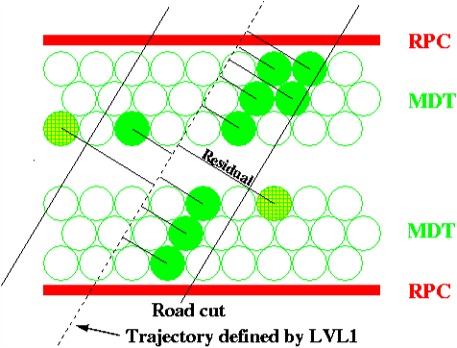
\includegraphics[clip, width=5.5cm]{fig/3/mdtResidual.png}
      \subcaption{各層で1つのMDTヒット選択の例}
      \label{fig:3-6-1}
  \end{minipage}
    \begin{minipage}[b]{0.5\linewidth}
      \centering
      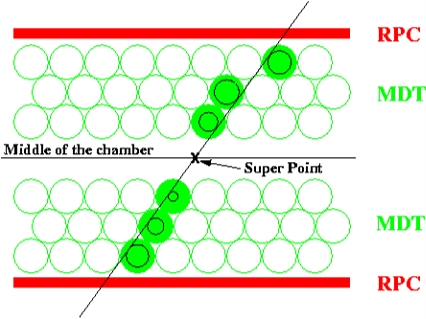
\includegraphics[clip, width=5.5cm]{fig/3/mdtRoad.png}
      \subcaption{ドリフト円のフィッティングからSPの求め方}
      \label{fig:3-6-2}
  \end{minipage}
  \caption{バレル領域におけるロードを用いたSPの求め方\cite{article:onlineMuonReconstruction}。}
\end{figure}

まず~RPCのヒットから求めたロードをもとに、MDTのヒットの選別を行う(図~\ref{fig:3-6-2})。ロード内の各~MDTヒットに対して、ロード中心からのドリフトチューブの距離~(residual)を計算し、各層について最もロード中心に近いチューブを選択することで各層から最大1つのヒットを用いる。
選択された各ヒットにおいてドリフト時間から距離を計算しドリフト円を定義し、その円のすべてに接する直線を仮定してフィットを行う。
最も$\chi^2$の小さい直線を各ステーションにおけるミューオンの飛跡とし、この飛跡と各ステーションのMDTチェンバーの中心線との交点を~SPの$r$、$z$座標とする。また、飛跡の傾きと切片を、SPの傾きと切片と定義する(図~\ref{fig:3-6-2})。


\subsubsection{部分飛跡を用いた$\pt$に相関のあるパラメータの導出}
ミューオンの$\pt$を求めるために、前段階で求めた~SPの傾きの情報を用いて$\pt$と相関のあるパラメータを計算する。

\paragraph{バレル領域における$\pt$と相関のあるパラメータの導出}
バレル領域では、インナー、ミドル、アウターステーションのすべてで磁場領域内に検出器が設置されているので、各ステーションのSPからミューオンの飛跡を再構成し、その曲率半径$R$を$\pt$と相関のあるパラメータとして定義する。
このとき、3つのステーションすべてで~SPを再構成できた場合は3点を用いて曲率半径を計算するが、3つの内2つのステーションのみでしか~SPを再構成できなかった場合は原点からインナーまで$z-R$平面でミューオンが曲がらずに飛んできたことを仮定して曲率半径を計算する。また1つのステーションのみでしか~SPを再構成できなかった場合は、曲率半径を計算できないので$\pt$の再構成を行わない。


\paragraph{エンドキャップ領域における$\pt$と相関のあるパラメータの導出}
エンドキャップ領域では、磁場領域内にインナーと~EE、ミドルステーションが、磁場領域外にアウターステーションが設置されている。
EEチェンバーが設置されている領域~($1.0<|\eta|<1.4$)では、インナーと~EE、ミドルステーションの~SPからミューオンの飛跡を再構成し、バレル領域と同様に曲率半径$R_{curv}$を$\pt$と相関のあるパラメータと定義する(図~\ref{fig:3-7})。
それ以外の領域では磁場領域内にステーションが2つしかなく、SPは最大2つしか再構成されないので曲率半径を計算することは不可能であるため、L2MuonSAでは磁場による飛跡の曲がりとして角度$\alpha$、$\beta$を定義する。$\alpha$、$\beta$は図~\ref{fig:3-8}と~\ref{fig:3-9}で表されるように定義される。

角度$\alpha$は図~\ref{fig:3-8}で表されるように、衝突点とミドルステーションの~SPの位置を結ぶ直線の傾きと、ミドルとアウターステーションの~SPを結ぶ直線の傾きのなす角である。アウターステーションに~SPがない場合はミドルステーションの~SPの傾きを用いる。
また~MDTから~SPを再構成できない場合は~TGCの情報を用いて$\alpha_{TGC}$を計算し、$\pt$再構成に用いる。

角度$\beta$は図~\ref{fig:3-9}で表されるように、インナーステーションでの~SPの傾きとミドル、アウターステーションの~SPを結んだ直線の傾きのなす角である。ここでも角度$\alpha$と同様にアウターステーションに~SPがない場合はミドルステーションの~SPの傾きを用いる。

\begin{figure}[h]
  \centering
  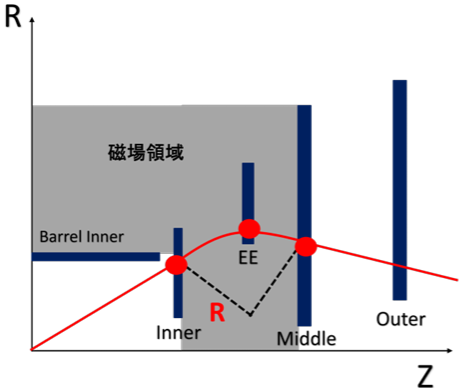
\includegraphics[clip, width=8cm]{fig/3/l2muonSA_Rcurv.png}
  \caption{エンドキャップ領域での~L2MuonSAにおける$R_{curv}$の定義\cite{article:noguchi}。}
  \label{fig:3-7}
\end{figure}

\begin{figure}[h]
  \centering
  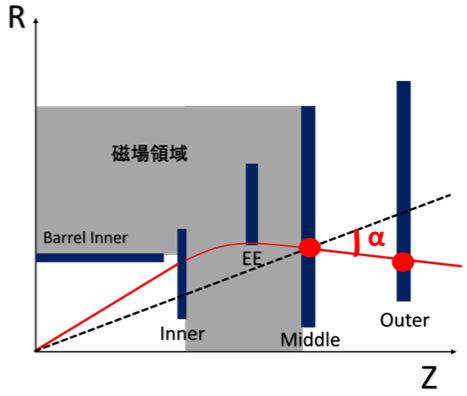
\includegraphics[clip, width=8cm]{fig/3/l2muonSA_alpha.png}
  \caption{エンドキャップ領域での~L2MuonSAにおける$\alpha$の定義\cite{article:noguchi}。}
  \label{fig:3-8}
\end{figure}

\begin{figure}[h]
  \centering
  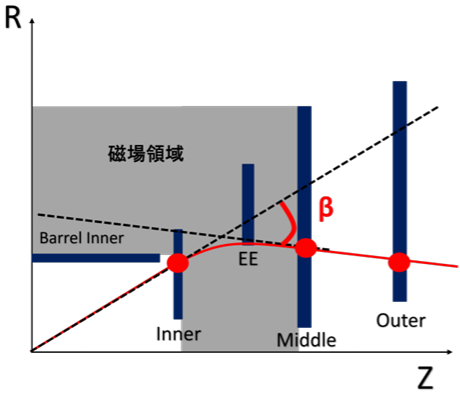
\includegraphics[clip, width=8cm]{fig/3/l2muonSA_beta.png}
  \caption{エンドキャップ領域での~L2MuonSAにおける$\beta$の定義\cite{article:noguchi}。}
  \label{fig:3-9}
\end{figure}



\subsubsection{Look~Up~Table~(LUT)を用いた$\pt$の導出}
全段階で求めた$\pt$と相関のあるパラメータから$\pt$を求める。
このとき高速で処理を行うために、あらかじめ$\pt$と相関のあるパラメータと$\pt$の対応表である~Look~Up~Table~(LUT)をメモリ上に用意しておき、参照することによって即座に$\pt$を導く。
ATLAS検出器では磁場の位置依存性があり、領域によってパラメータと$\pt$の相関は異なるので、セクターや荷電粒子の電荷や、$\eta$、$\phi$などで細かく分割された領域ごとに~LUTを作成している。

\paragraph{バレル領域における~LUTを用いた$\pt$の導出手法}
バレル領域では、$\rm{sector}\times Q \times \eta \times \phi = 4\times2\times30\times30$に領域を分割し、それぞれの領域で~LUTが作成されている。
sectorは~Large、Small、Large~Special、Small~Specialステーションの4分割、$Q$は荷電粒子の電荷、$\eta$、$\phi$方向はセクターにより異なる範囲で30分割している。
$\eta$、$\phi$方向の30分割する範囲を以下に示す。
\begin{itemize}
    \item Largeセクター~:~$-1.145<\eta<1.145、-0.230<\phi<0.230$
    \item Smallセクター~:~$-1.050<\eta<1.050、-0.181<\phi<0.181$
\end{itemize}


各領域ごとの飛跡の曲率$R_{curv}$と$\pt$の相関は以下の式で表される。
\begin{equation}
    p_{\mathrm{T}}=A \times R_{curv}+B
\end{equation}
この式における$A$、$B$を前もってデータから求めてLUTにまとめることで、飛跡の領域と$R_{curv}$から$\pt$を求める。


\paragraph{エンドキャップ領域における~LUTを用いた$\pt$の導出手法}
エンドキャップ領域では、$\eta \times \phi \times (Q \times \eta/|\eta|)= 30\times12\times2$に領域を分割し、それぞれの領域で~LUTが作成されている。$Q$は荷電粒子の電荷で、$\eta/|\eta|$は~A、C-sideを表す。
$\eta$方向はエンドキャップ領域の$1.05<|\eta|<2.50$の範囲で$|\eta|$を30分割、$\phi$方向は$\phi$全体の領域で8回対称を仮定し、さらにそれぞれの線対称を仮定した後に~Large~sectorの中心から~Small~sectorの中心までを12分割している(図~\ref{fig:3-10})。

\begin{figure}[h]
  \centering
  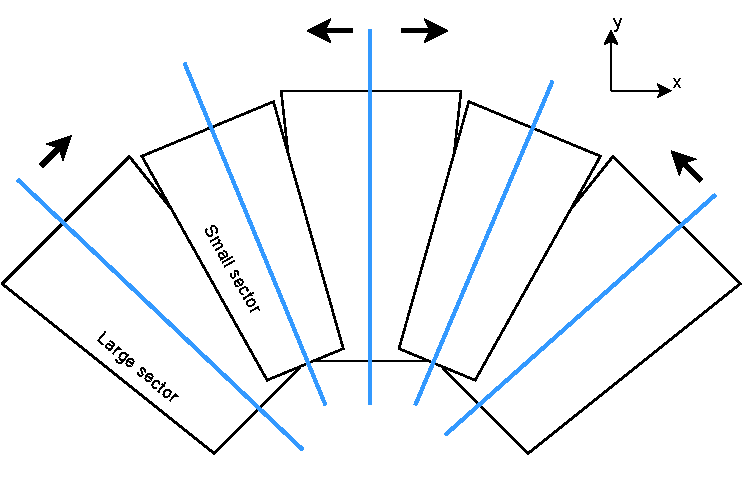
\includegraphics[clip, width=10cm]{fig/3/LUT_binning.pdf}
  \caption{エンドキャップ領域での$\phi$の領域分割の定義。}
  \label{fig:3-10}
\end{figure}

各領域ごとの$\alpha$、$\beta$、$1/R_{curv}$と$\pt$の相関は以下の式で表される。
\begin{equation}
    \alpha, \beta, 1 / R_{\text {curv }}=A \times\left(\frac{1}{\pt}\right)+B \times\left(\frac{1}{\pt}\right)^2
\end{equation}
この式における$A$、$B$を前もってデータから求めてLUTにまとめることで、飛跡の領域と$\alpha$、$\beta$、$1/R_{curv}$から$\pt$を求める。
$A$、$B$から$\pt$の値への変換は以下の式を用いる。

\begin{equation}
    \frac{1}{\pt}=\frac{-A+\sqrt{A^2+4 B\left(\alpha, \beta, 1 / R_{\text {curv }}\right)}}{2 B}
\end{equation}

$R_{curv}$、$\alpha$、$\beta$それぞれから$\pt$を算出するが、実際にL2MuonSAの$\pt$は1つ選択される。
$R_{curv}$、$\alpha$、$\alpha_{TGC}$、$\beta$から計算された$\pt$をそれぞれ$p_{\mathrm{T},R_{curv}}$、$\ptAlpha$、$p_{\mathrm{T,TGC}}$、$\ptBeta$と表す。
この中では磁場内に設置されている検出器3つを用いて求めた$p_{\mathrm{T},R_{curv}}$が最も精度が良い。
そのため$R_{curv}$が計算できた場合は優先的に$p_{\mathrm{T},R_{curv}}$を使用する。

$\ptAlpha$は衝突点からインナーステーションまでミューオンが曲がらずに飛んでいることを仮定しているが、実際にはカロリメータ等による多重散乱によって飛跡が曲げられることがある。
そのためインナーステーションを使用する$\ptBeta$の方が原理的には分解能がいいはずである。
しかし$\beta$はミドルステーションとアウターステーションに加えてインナーステーションのSPの情報を用いるので、インナーステーションでのSPの再構成の誤差が大きければ$\pt$の再構成を間違える割合が増える。
インナーステーションはミューオン検出器の最内層でカロリメータのすぐ外側に位置し、カロリメータから漏れ出てくるミューオン以外の荷電粒子の数が多い。
これがミューオンからの検出器信号と重なると、$\pt$の計算を間違える場合が多い。
そのため$R_{curv}$による$\pt$の計算ができない場合は、$\pt$を使い分ける必要がある。

$\pt$の選択方法について、図~\ref{fig:3-11}に示す。
$\ptBeta$単独で値が正しいかどうかの判定をすることは困難なので、$\ptAlpha$の値と比較して値のずれが小さければ$\ptBeta$が信頼できる値であること、$\ptBeta$がずれているときは$\ptBeta$が低くなることが多いことなどを用いて、$\pt$の選択を行う。

\begin{figure}[h]
  \centering
  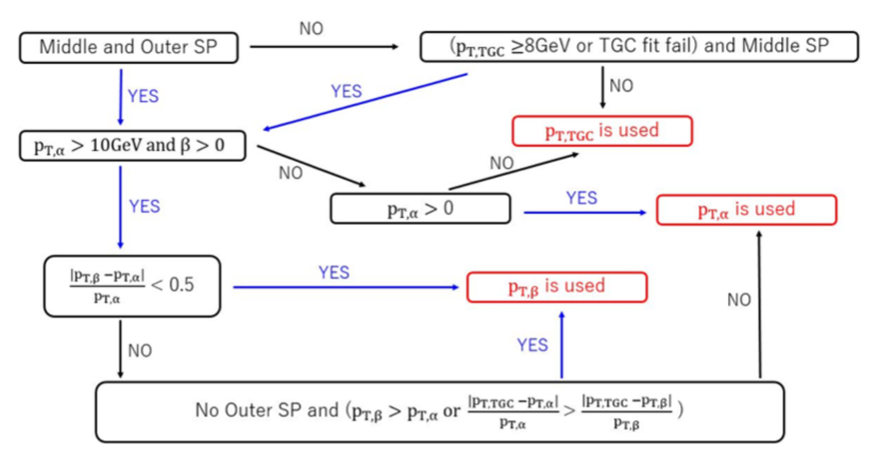
\includegraphics[clip, width=14cm]{fig/3/l2muonSA_pTselection.png}
  \caption{エンドキャップ領域でのL2MuonSAにおける$p_{\mathrm{T},R_{curv}}$、$\ptAlpha$、$\ptBeta$、$p_{\mathrm{T,TGC}}$の選択条件\cite{article:wakamiya}。}
  \label{fig:3-11}
\end{figure}


\subsection{Level2~Combined~Muon~(L2MuComb)}\label{chapter3-2-3}
Level-2~Combined~Muon~(L2MuComb)では、L2MuonSAで計算した飛跡と内部飛跡検出器の情報を組み合わせてミューオンの$\pt$の再構成を行い、トリガー判定を行う。
まず、L2MuonSAで再構成した飛跡を内部飛跡検出器の位置まで外挿する。
外挿された飛跡の周辺で、内部飛跡検出器で測定されたミューオン候補の飛跡を探索する。
見つかったミューオン候補の飛跡とL2MuonSAの飛跡の$\chi^2$を$\eta$、$\phi$、$\pt$などの情報を用いて計算し、最も$\chi^2$の小さい飛跡の$\pt^{ID}$を取得する。
この$\pt^{ID}$とL2MuonSAの$\pt^{SA}$で、分解能に基づく重み~($w^{SA}$、$w^{ID}$)を用いて加重平均を取ることでL2MuCombにおける$\pt^{CB}$を計算する。

\begin{equation}
    \frac{1}{\pt^{C B}}=\frac{w^{S A} \cdot \frac{1}{\pt^{S A}}+w^{I D} \cdot \frac{1}{\pt^{I D}}}{w^{S A}+w^{I D}}
\end{equation}

\subsection{Event~Filter~(MounEF)}\label{chapter3-2-4}
Event~Filter~(EF)では、全検出器の情報を用いてミューオンの飛跡を再構成する。
再構成アルゴリズムはオフライン再構成アルゴリズムとほとんど同じものを用いるので、精密な飛跡の再構成を行うことが可能である。
$Z\rightarrow\mu\mu$のような2つのミューオン同士が離れているような物理現象を検出対象としたミューオントリガーでは、ミューオンの内部飛跡検出器での飛跡の周辺に他のミューオンが存在しないこと~(アイソレーション)を要求して選別も行う。
このような$\pt$以外の要求による選別は、$\pt$の閾値を低くした場合のバックグラウンドを削減でき、トリガーレートを抑制できるため、低い$\pt$のミューオンを含む事象を取得するために有用である。

\subsection{ミューオントリガーチェーン}\label{chapter3-2-5}
ミューオントリガーは基本的に、L1、MuonSA、MuonCB、EFの判定を組み合わせることによって構成される。
各段階のトリガーを組み合わせたものをトリガーチェーンと呼ぶ。後段のトリガーほど$\pt$再構成の精度が良くなるので、後段のトリガーほど厳しい$\pt$の閾値が設定されている。
トリガーチェーンは検出対象の物理に合わせて、様々な$\pt$しきい値の各トリガーを組み合わせて用いられている。


\subsection{オフライン再構成}\label{chapter3-2-6}
トリガーを通過してデータに記録された事象に対して、もう一度全検出器の情報の用いてミューオンの再構成を行うことをオフライン再構成と呼ぶ。
トリガー稼働中とは異なり時間の制限がないため、より正確に飛跡を再構成することができる。
オフラインミューオン再構成では複数のアルゴリズムを用いており、主なものはミューオン検出器の情報のみを用いて再構成を行う~Stand~Aloneミューオン~(SA)と、ミューオン検出器と内部飛跡検出器の情報を合わせて再構成を行う~Combinedミューオンである。
SAの利点として衝突点由来でないミューオンを再構成できることがある。
%SAの利点は、内部飛跡検出器が存在しない$|\eta|>2.5$の領域でもミューオンの飛跡を再構成できることである。


\newpage

\section{第3期運転~(Run-3)における新ミューオントリガーアルゴリズム}\label{chapter3-3}
2014年から2022年までのロングシャットダウンを経て、2022年から第3期運転~(~Run-3)が開始された。
Run-3から新たに様々なトリガーが導入されたが、本論文では2つのミューオントリガーについて取り上げる。

\subsection{近接2ミューオンのためのトリガーアルゴリズム}\label{chapter3-3-1}
Run-2まで、2ミューオントリガーは2つのミューオンが近接している時に検出効率が低下してしまうという問題点があった。
図~\ref{fig:3-12}にバレル領域における2ミューオントリガーのトリガー効率を示す。

\begin{figure}[H]
    \centering
    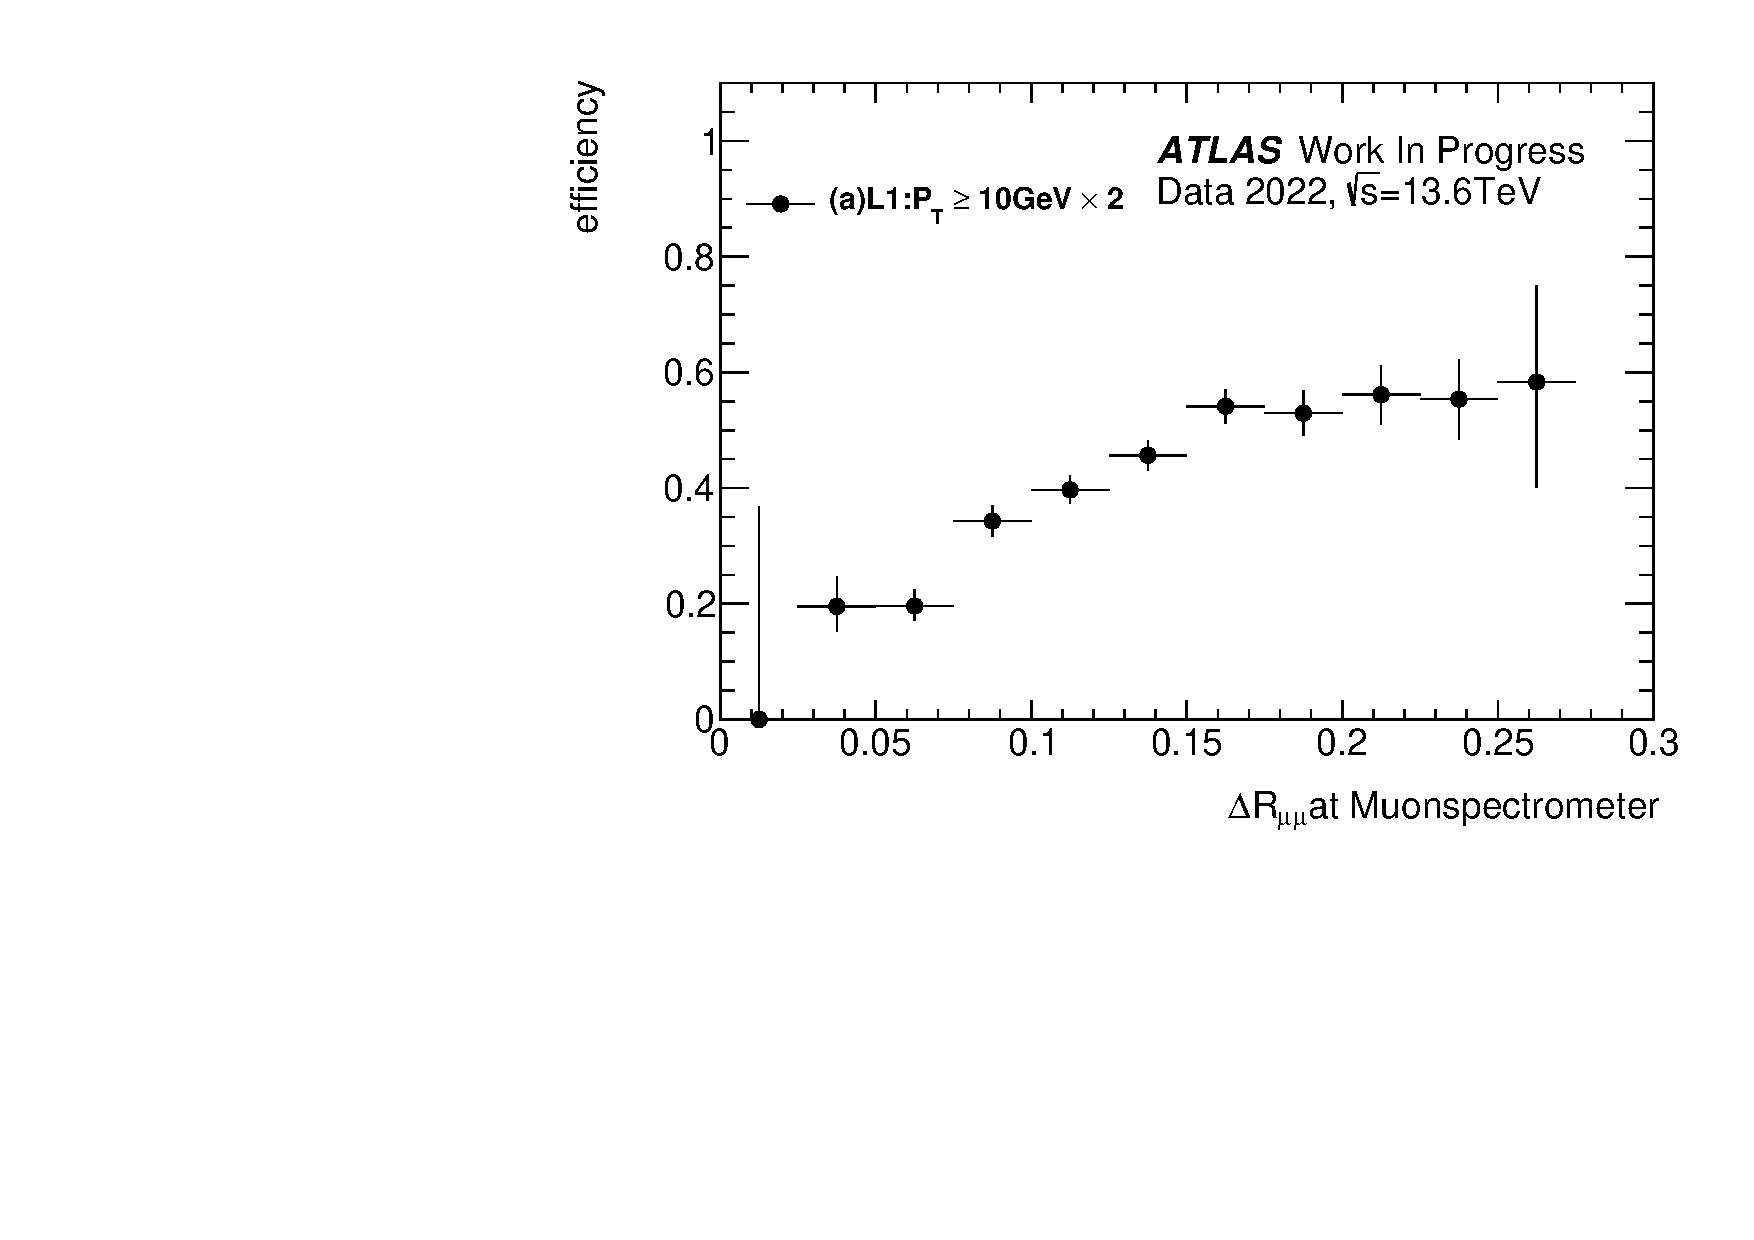
\includegraphics[clip, width=12cm]{fig/3/L1_2MU10_eff.pdf}
    \caption{バレル領域における~L1の2ミューオントリガーを通過することが期待される事象に対する、L1の2ミューオントリガー効率}
    \label{fig:3-12}
\end{figure}

\begin{figure}[H]
    \centering
    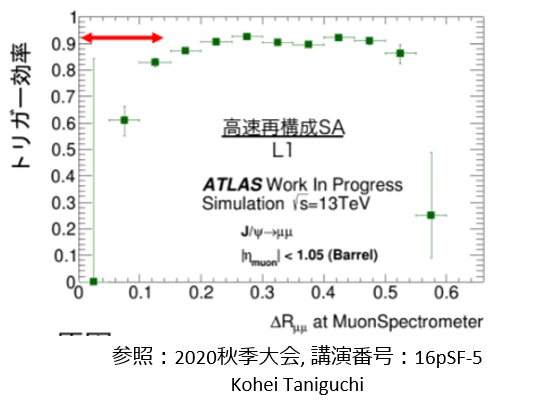
\includegraphics[clip, width=12cm]{fig/3/l2saEff_taniguchi.png}
    \caption{バレル領域におけるL1の2ミューオントリガーを通過した事象に対する、MuonSAの2ミューオントリガーの効率}
    \label{fig:3-13}
\end{figure}

ここで$\eta$と$\phi$の値から計算される、2つのミューオンの飛跡同士の距離を示す$\Delta R_{\mu\mu}$という値を以下の式で定義する。

\begin{equation}
    \Delta R_{\mu \mu}=\sqrt{\left(\eta_{\mu 1}-\eta_{\mu 2}\right)^2+\left(\phi_{\mu 1}-\phi_{\mu 2}\right)^2}
\end{equation}

衝突点での2ミューオン同士の$\Delta R$を$R_{\mathrm{~at~vertex}}$, 衝突点でのミューオンの$\eta$、$\phi$をミューオン検出器のあるミドルステーションの位置まで外挿した値を用いて計算するミューオン検出器での$\Delta R$を$R_{\mathrm{~at~Muon~Spectrometer~(MS)}}$と定義する。

図~\ref{fig:3-12}から2つのミューオン同士が非常に近接する$\Delta \mathrm{R}$が0.15以下の領域において、L1・HLTともにトリガー効率が顕著に低下していることがわかる。

2ミューオントリガーの2ミューオンが非常に近接している領域におけるトリガー効率の低下は、L1でミューオンの通過位置を表す最小単位である~RoIは1つの~Padにつき1つしか出力できず、また1~Padのサイズが$\Delta\eta\times\Delta\phi=0.2\times0.2$と大きいので2つのミューオンが同一~Padを通過した場合L1で2ミューオントリガーでは検出できないことが原因であった。
また、従来の~L2MuonSAアルゴリズムでは1つの~RoIから1つのミューオンしか再構成できなかったため2ミューオンが非常に近接している領域ではトリガー効率が低下してしまっていた。

そこで先行研究\cite{article:taniguchi}において、1つの~RoIから複数のミューオンを再構成することができる~L2MuonSAアルゴリズムが新たに開発された(谷口浩平, 2021)。


\subsection{NSWを用いたL2MuonSAでの部分飛跡再構成アルゴリズム}\label{chapter3-3-2}
第2章で述べたように、NSWは~Run-3から~LHCのルミノシティ増加に伴い検出器のヒットレートが増加することに対応するために導入された検出器である。
LHCの最高瞬間ルミノシティは、Run-3の期間内に$2~3\times10^{34}cm^{-2}s^{^1}$に到達し、2025年からのロングシャットダウン期間に更なるアップグレードを経て$5\times10^{34}cm^{-2}s^{-1}$を実現する予定である。
LHCのルミノシティ増加により、パイルアップや背景事象が増加し検出器へのヒットレートが増加する。Run-2までエンドキャップ領域のインナーステーションに配置されていた~Small~Wheel~(SW)では増加したヒットレートに耐えることができず、トラッキング性能が低下する。このことに対応するために~NSWが導入された。

\begin{figure}[H]
    \centering
    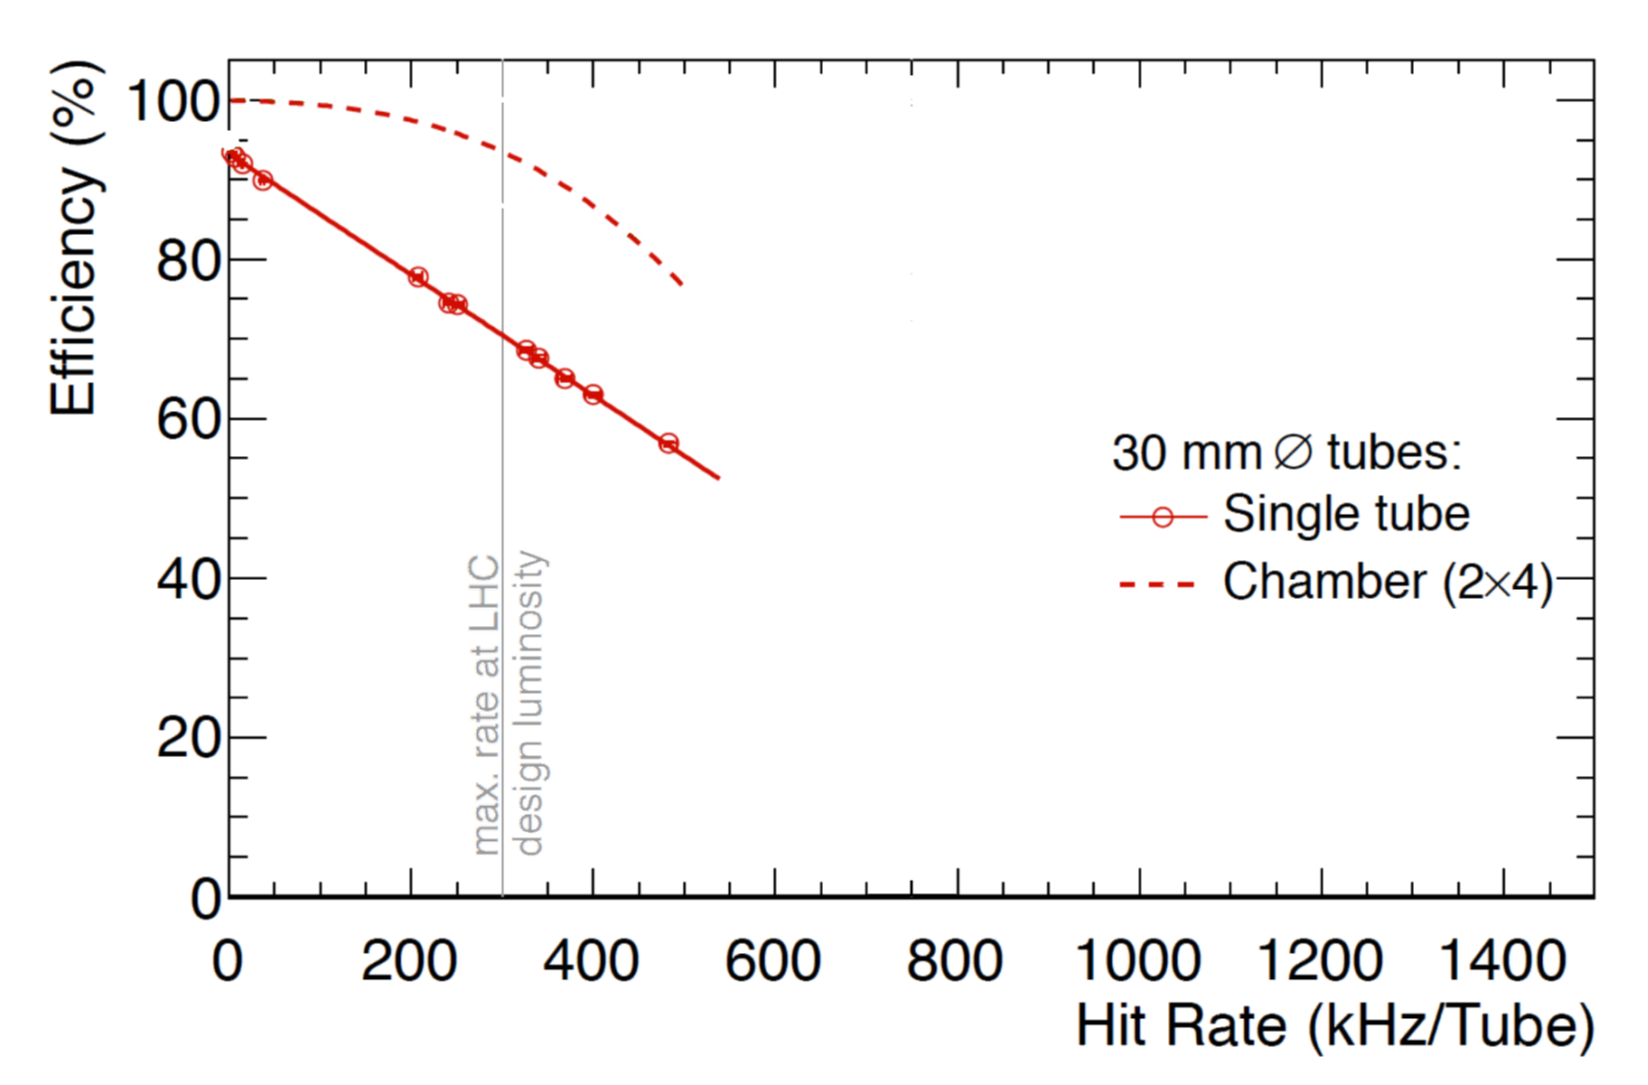
\includegraphics[clip, width=10cm]{fig/3/NSW_HitRate.png}
    \caption{MDTの1チューブ当たりのヒットレートとefficiencyの関係。実線が1チューブに対するefficiencyで破線がチェンバーに対するefficiencyである\cite{article:ATLASNSWTDR}}
    \label{fig:3-14}
\end{figure}


NSWはミューオントリガーにも用いられる。
HLTでも~NSWを用いて部分飛跡を再構成するアルゴリズムが開発され、Run-3の運用が始まる前にシミュレーションでの性能評価を経て導入された。

\subsection{本論文の目的}\label{chapter3-4}
新しく導入されたトリガーは、シミュレーションでその性能が評価されているが実際に検出器を動かしたときの性能は評価されていない。実際にトリガーを用いてデータを選別して取得し、物理解析に用いるためにはそのトリガーが正しく、想定通りの動作をしていることを確認する必要がある。
本研究では近接2ミューオンのためのトリガーと新たに導入された検出器~NSWを用いた~L2MuonSAアルゴリズムについて、Run-3実データを用いて動作検証を行った。
近接2ミューオンのために改良されたトリガーのアルゴリズムの詳細な説明と、実際に~Run-3において取得したデータを用いて行ったトリガーの性能評価について第4章で述べる。
また第5章で~NSWを用いた~L2MuonSAアルゴリズムの詳細な説明と、Run-3実データを用いた検証結果について述べる。
実データでの検証の結果、シミュレーションから想定されていた動作と大きく異なる点が見つかった。
そのことに対応するために新たに検討した~L2MuonSAアルゴリズムとその評価についても述べる。